\chapter{Wprowadzenie}
\label{cha:wprowadzenie}

Jesteśmy obecnie świadkami rozrostu miast, budowy kompleksów sportowych czy galerii handlowych. Wszystkie te miejsca są nieodłącznie związane z tłumami przewijających się przez nie osób. W związku z rosnącą gęstością zaludnienia oraz wzrostem zagorzeń takich jak terroryzm tworzenie symulacji ewakuacji nabrało większego znaczenia.\\

W ostatnich dekadzach ilość wypadków związanych ze złym planowaniem ewakucaji wzrosła. Katastrosy takie jak tragedia w Hillsborough w roku 1989 (96 ofiar) czy wybuch paniki na Love Parade w Duisburgu w roku 2010 (21 ofiar) pokazują, że efektywność ewakuacji stała się kluczowym aspektem bezpieczeństwa w miejscach publicznych takich jak stadiony, stacje metra czy lotniska. Symulacje mogą mieć wielorakie zastosowanie, począwszy od wspomnianej ewakucaji ludności poprzez badanie zachowań w centrach handlowych kończąc na ruchu drogowym. Dzięki zasymulowaniu zachowania tłumu możemy łatwiej utworzyć plany ewakuacyjne na wypadek zagrożenia minimalizując szkody oraz ofiary. Pozwalają one także na lepsze rozładowanie ruchu drogowego w miastach o rosnącej gestości zaludnienia. \\

Na przejściach dla pieszych w Japonii ginie 30\% osób uczestniczących w wypadkach drogowych \cite{AMSFMfPBSaSC}, a w Niemczech odsetek ten wynosi 15\% \ [German instigute for econeomic research 2010]. Zgodnie z danymi organizacji Fire Administration w Stanach Zjednoczonych \cite{Asfemwle} w roku 2007 3430 osób zmarło w pożarach oraz blisko 18 tysięcy zostało rannych. Biorąc pod uwagę te dane łatwo dojść do wniosku jakie korzyści mogą płynąć z symulacji zachowania pieszych.

Zachowanie tłumu badane jest od przeszło trzech dekad. Na samym początku badania były traktowane w ramach ciekawostki. W ostatnich czasach symulacje ruchu pieszych zyskały na popularności. Głównie za sprawą analogii do zachowania gazów oraz płynów \cite{SforceModelForPedDyn}. Wraz z nowatorskimi pracami Helbinga .... .  Modelowanie ruchu pieszych odgrywa ponadto dużą rolę w projektowaniu, dostarcza wielu informacji użytecznych podczas planowania miejsc użyteczności publicznej. Znajomość problemów podczas ewakuacji, sytuacji konfliktowych pomiędzy pieszymi jest kluczowa w projektowaniu nowych budynków. W przypadku małych budynków łatwo można przeprowadzić próbne ewakuacje, jednakże kiedy w grę wchodzą duże kompleksy nie jest to możliwe. Nawet próba z małą ilością osób nie pokaże skali problemu. Nie jesteśmy wówczas w stanie przykładowo zbadać jak na ewakuacje wpłynie rosnąca gęstość tłumu.

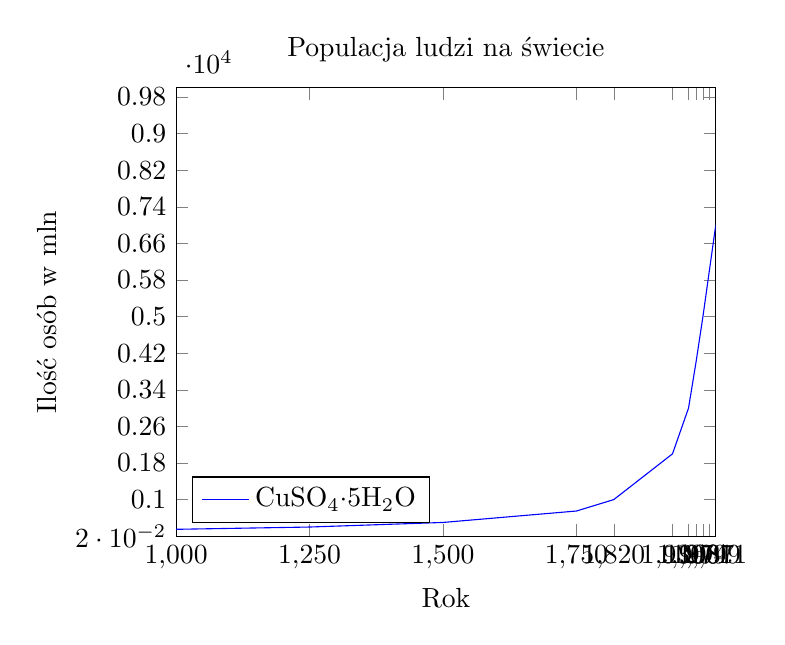
\begin{tikzpicture}
\begin{axis}[
    title={Populacja ludzi na świecie},
    xlabel={Rok},
    ylabel={Ilość osób w mln},
    domain=1000:2011,
    xmin=1000, xmax=2011,
    ymin=200, ymax=10000,
    xtick={1000,1250,1500,1750,1820,1930,1960,1974,1987,1999,2011},
    ytick={200,1000,1800,2600,3400,4200,5000,5800,6600,7400,8200,9000,9800},
    legend pos=south west,
]
 
\addplot[
    color=blue,
    ]
    coordinates {
    (1000,350)(1250,400)(1500,500)(1750,750)(1820,1000)(1930,2000)(1960,3000)(1974,4000)(1987,5000)(1999,6000)(2011,7000)
    };
    \legend{CuSO$_4\cdot$5H$_2$O}
 
\end{axis}
\end{tikzpicture}
%---------------------------------------------------------------------------

\section{Cele pracy}
\label{sec:celePracy}

Głównym celem pracy jest implementacja oraz zasymulowanie zachowania pieszych używając metody Social Force. Symulacja ruchu pieszych skupia się na zbadaniu zachowania ludzi dla dużych populacji w małych przestrzeniach. Zaproponowany model pozwala na opisanie każdej osoby z osobna biorąc pod uwagę jej indywidualne cechy takie jak prędkość ruchu czy masę. Symulacja bierze pod uwagę także aspekty psychologiczne oraz socjologiczne jakie można nakreślić badając zachowanie tłumu

%---------------------------------------------------------------------------

\section{Zawartość pracy}
\label{sec:zawartoscPracy}

Rozdział 1,~\ref{cha:wprowadzenie}: przedstawiono podstawowe informacje dotyczące symulacji komputerowych z ruchem pieszych. Kolejny rozdział poświęcony jest porównaniu istniejących rozwiązań pomagających takie symulacje zaimplemnetować.

Rozdział 2, \ref{cha:wprowadzenieTeoretyczne}: nakreślone zostają teoretyczne askepty symulacji

\section{Zastosowanie symulacji komputerowych}
\label{sec:ZastosowanieSymulacji}


















